% Created 2019-05-16 jue 21:30
% Intended LaTeX compiler: pdflatex
\documentclass[11pt]{article}
\usepackage[utf8]{inputenc}
\usepackage[T1]{fontenc}
\usepackage{graphicx}
\usepackage{grffile}
\usepackage{longtable}
\usepackage{wrapfig}
\usepackage{rotating}
\usepackage[normalem]{ulem}
\usepackage{amsmath}
\usepackage{textcomp}
\usepackage{amssymb}
\usepackage{capt-of}
\usepackage{hyperref}
\author{Marco Centurion}
\date{\today}
\title{Installation Guide}
\hypersetup{
 pdfauthor={Marco Centurion},
 pdftitle={Installation Guide},
 pdfkeywords={},
 pdfsubject={},
 pdfcreator={Emacs 26.1 (Org mode 9.1.9)}, 
 pdflang={English}}
\begin{document}

\maketitle
\tableofcontents

\section{Description}
\label{sec:org5c161cf}

This document explains the steps needed to install the software developed in the context of the thesis "Model Driven Engineering applied to Network Configuration".

\section{Dependencies}
\label{sec:org4b39ff3}

In order to install this software, you must have an installation of Eclipse Development Tools, with some extra plug-ins. 

\subsection{Summary}
\label{sec:org2f21645}

As a summary, you need the following environment configurations:

\begin{itemize}
\item \texttt{Eclipse Modeling Tools} \footnote{\href{https://www.eclipse.org/downloads/packages/release/2008-09/r/eclipse-modeling-tools}{Download link for Eclipse Modeling Tools}} 2018-09
\item \texttt{Papyrus} \footnote{\href{https://www.eclipse.org/papyrus/}{Papyrus main web page}} 4.1.0.201809120950
\item \texttt{Acceleo} \footnote{\href{https://www.eclipse.org/acceleo/}{Acceleo project main web page}} 3.7.8.201902261618
\end{itemize}

The referenced versions are the latest ones in which the software was tested, we cannot guarantee that the software will work properly in newer releases.

\subsection{Eclipse}
\label{sec:org721ce9f}

Regarding \texttt{Eclipse's} installation, we suggest you use the tool \texttt{Eclipse Oomph}\footnote{\href{https://projects.eclipse.org/projects/tools.oomph}{Eclipse Oomph main web page}}. After downloading \texttt{Oomph}, you can run it,
which will show the following window, at this point you should select \texttt{Eclipse Modeling Tools}:

\begin{center}
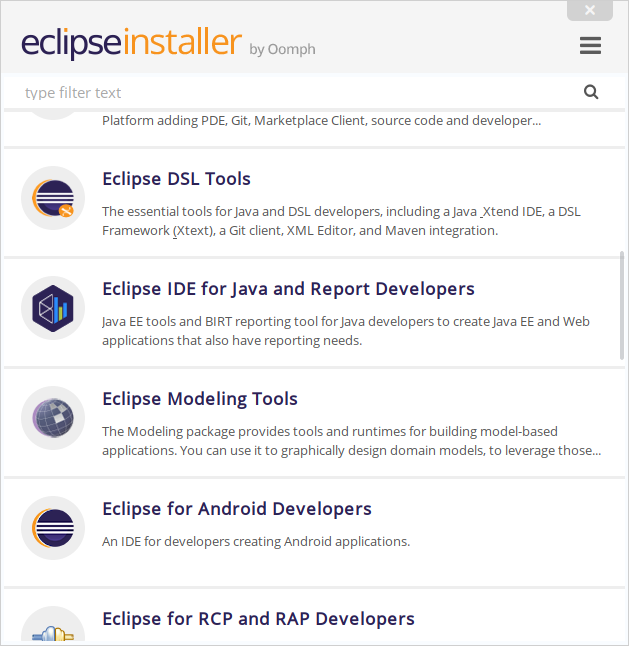
\includegraphics[width=.9\linewidth]{images/oomph_main.png}
\end{center}

In the next window you must select version \texttt{2018-09}:

\begin{center}
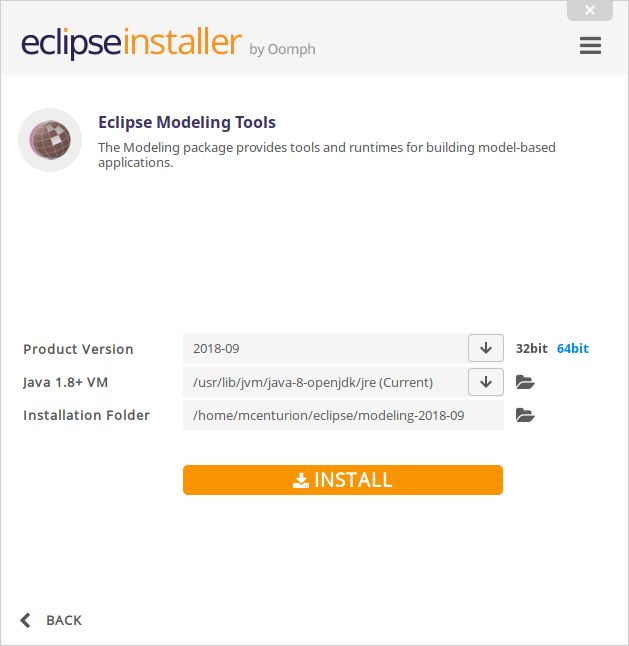
\includegraphics[width=.9\linewidth]{images/oomph_selection.png}
\end{center}

Clicking \texttt{Install} will begin the installation, during this process you may need to accept several licenses in order to proceed.

Once the installation is complete, \texttt{Oomph} will allow you to execute \texttt{Eclipse}:

\begin{center}
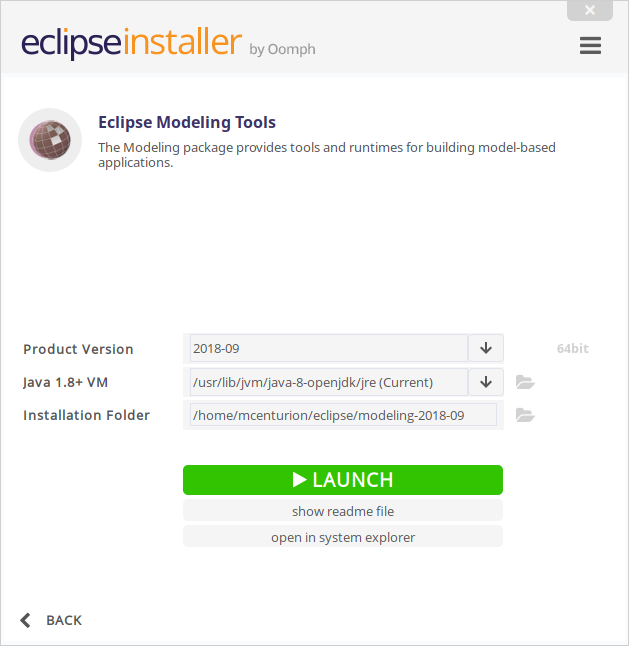
\includegraphics[width=.9\linewidth]{images/oomph_launch.png}
\end{center}

This will finish the installation.

\subsection{Libraries}
\label{sec:org82d9ff1}

All the libraries that need to be installed can be found in Eclipse's default repositories. 

\subsubsection{Papyrus}
\label{sec:orgedb7b37}

\texttt{Papyrus} can be installed from the software installation window in \texttt{Eclipse}, which you can find under "Help > Install New Software\ldots{}".

By choosing "--All Available Sites--" as source, you can easily find \texttt{Papyrus for UML} under the "Modeling" category:

\begin{center}
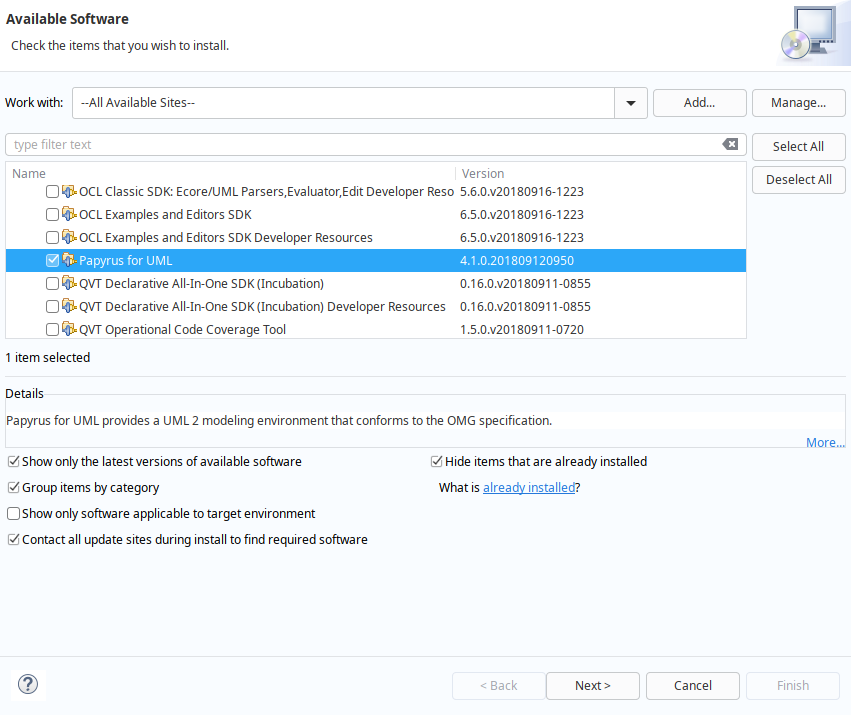
\includegraphics[width=.9\linewidth]{images/papyrus.png}
\end{center}

After you select that option, you can continue with the installation process, where you must once again accept all licenses presented.

To finish the installation of \texttt{Papyrus}, you will need to restart
\texttt{Eclipse}. You can ignore this step if you are also going to install \texttt{Acceleo} at this moment.

\subsubsection{Acceleo}
\label{sec:orgfd3943c}

\texttt{Acceleo} cannot be installed from the software installation window as \texttt{Papyrus}, but it can be installed from \texttt{Eclipse Marketplace},
found at "Help > Eclipse Marketplace\ldots{}".

Once the marketplace is open, you can find \texttt{Acceleo} using the search field, and then install it clicking the "Install" button.

\begin{center}
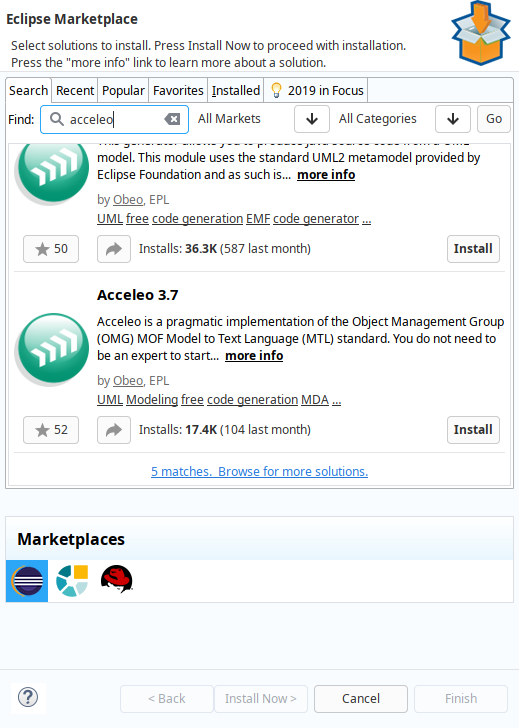
\includegraphics[width=.9\linewidth]{images/acceleo.png}
\end{center}

In the same way as \texttt{Papyrus}, you must proceed with the installation process, and at the end you will need to restart \texttt{Eclipse}.

\section{Installation}
\label{sec:orgb6f475c}

The steps to install the developed plug-in are very straightforward.

First of all, you need to have all the required plug-ins:

\begin{itemize}
\item mdcms plug-in: provides the UML profile.
\item mdcms2puppet plug-in: provides the model to text transformation, from mdcms to puppet code.
\item mdcms2puppet-ui plug-in: adds the UI element to the right click menu on .uml files.
\end{itemize}

In order to install these plug-ins, you just need to:

\begin{enumerate}
\item Find \texttt{Eclipse} installation directory.
\item Find the directory named "dropins".
\item Copy all .jar files from the plug-ins to the "dropins" directory.
\item Start \texttt{Eclipse}.
\end{enumerate}

After executing \texttt{Eclipse} you can verify that the plug-ins were installed correctly by navigating to "Help > About Eclipse IDE > Installation
Details", and search for them on the tab "Plugins".

\begin{center}
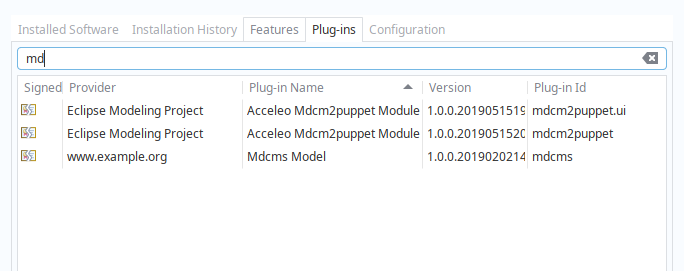
\includegraphics[width=.9\linewidth]{images/plugins.png}
\end{center}
\end{document}
